\documentclass{article}

\usepackage{stdheader}
\graphicspath{{../figs/}}

\DeclareMathOperator\Tr{Tr}

\title{The Berry Phase}
\author{Jacob MacWilliams}
\begin{document}

\maketitle
\tableofcontents

\newpage
\section{Introduction \label{sec:intro}}

It has long been known that the global phase of a quantum state was physically irrelevant. The standard argument goes that all measurements in the quantum mechanical realm can be modelled as Hermitian operators ($\hat{O}$), which in turn can be represented in their spectral decomposition ($\hat{O} = \sum_{i} \omega_{i}\ket{\Psi_i}\bra{\Psi_i}$) which are in turn gauge-invariant with respect to gauge transformation of the type:

\begin{equation*}
  \mathcal{G}: \mathcal{H} \rightarrow \mathcal{H}^{*} \quad  \ket{\Psi} \mapsto e^{i\alpha(\Psi)}\ket{\Psi}
\end{equation*}

It would be naive to extrapolate this argument too far and assume that phase is wholly irrelevant to quantum systems. It has been clear since the inception of quantum mechanics that this is not the case, and that the relative phase between two states can plays a crucial role in a system's behaviour. However, perhaps slightly more surprising is that the Hilbert space of a system, itself, shields certain internal phase relations within it from changing under arbitrary gauge transformations. It was Michael Berry in 1983 that discovered that quantum systems transported slowly around a circuit by varying some control parameters $\bm{R}$ exhibit a phase factor which he dubbed the \textit{geometric phase} \cite{Berry1984}. In the same year Barry Simon made the connection between Berry's geometric phase and topology showing that the phase is a result of the geometry of the parameter space \cite{Simon1983}. With this discovery, the quantum world was intimately connected with the worlds of geometry and topology, and the gates to the study of quantum systems through the lens of topology/geometry was opened.\\

This report will focus on only the beginning of this story; that being an introduction and exploration of the geometric phase, now more often called The Berry Phase\footnote{Following Berry's discovery of his self-dubbed geometric phase in 1983 and Simon's consequent generalization further generalizations were made such as the introduction of The Aharonov-Anandan Phase in 1986. As time progressed further connections were made to a variety of phase factors found in other fields of physics. All of these phase factors could be reasonably called geometric phase factors, and using the same term for all of them would not be in of itself incorrect as they are all inherently connected by the same mathematical concepts, but called differently because the various histories of these independent discoveries. So, to avoid confusion I will be using the term Berry Phase, meaning the geometric phase factor discovered by Michael Berry in the context of the quantum physics.}.  In this report I will derive The Berry Phase in a manner inherently intertwined with Simon's insights\ref{sec:SECTION}, exploring its properties \ref{sec:SECTION}, and then going on to detail the theoretical arguments through which Berry unveiled The Berry Phase. In the final section of the body of this report a number of physical systems will be explored in which The Berry Phase arises, during which a numerical solution will be presented showing The Berry Phase arising in a physical model as one would expect.\\

I urge the reader to keep in mind that the relevance of this report derives itself from the importance of the much larger field of topological physics and the role The Berry Phase plays in connecting the quantum realm to the realm of topology. Understanding The Berry Phase in this context provides a natural jumping off point into a much wider world with a whole array of interesting phenomena and insights.

\section{The Berry Phase\label{sec:the_berry_phase}}

\subsection{The Discrete Case \label{ssec:discrete_case}}

In this section The Berry Phase will be introduced in the discrete case; that is, it will be defined for a Hilbert space ($\mathcal{H}$) with a finite number of states ($N$). \\ 

Before introducing The Berry Phase we first have to define the relative phase between two states ($\ket{\Psi_1}$, $\ket{\Psi_2}$):

  \begin{equation*} \label{eq:relative_phase}
    \gamma_{1,2} = -arg \braket{\Psi_{1}|\Psi_{2}} \qquad \gamma_{1, 2} \in (-\pi, \pi]
  \end{equation*}

That being the phase factor of the complex number describing the inner product of the two states with each other. Here the total range of values allowed for the phase is restricted, respecting the equivalence of values outside this range under the relation $\gamma_{0} \equiv \gamma_{1} \Leftrightarrow e^{i\gamma_{0}} = e^{i\gamma_{1}}$. One can quickly show that this phase factor itself is not of any physical relevance as it is expressly dependent on our initial choice of a gauge:

  \begin{equation*}
    \ket{\Psi_{j}} \rightarrow \exp(i \alpha_{j}) \ket{\Psi_{j}} \quad\quad
    \exp(-i\gamma_{1,2}) \rightarrow \exp(-i\gamma_{1,2} + i(\alpha_{2} - \alpha_{1}))\\
  \end{equation*}

Restricting ourselves now, for the sake of simplicity, to a finite Hilbert space (an $N$-state system) one can define the loop/Berry phase\footnote{For all intents and purposes the loop phase is The Berry Phase in the discrete case. However as the loop phase is not the phase as Michael Berry discovered it, and as a number of other phase factors in the literature are inherently the same though they are named differently (as I discussed in the previous footnote) I will refrain from calling the loop phase, The Berry Phase here.} along any given \textit{loop} $c_m=[n_{0}, n_{1}, \ldots, n_{m}, n_{m+1}], \quad n_{0} = n_{m+1}$ (Fig: \ref{fig:berry_loop}):

  \begin{equation*}
    \gamma_{L}(c_m) = \sum_{i \leq m}\gamma_{n_{i}, n_{i+1}}
  \end{equation*}

Applying a general gauge transformation ($\mathcal{G}$) to the Hilbert space in which our states live we can utilize the transformation properties of the relative phase (Eq: \ref{eq:relative_phase}) to show that the loop phase over an arbitrary sequence defining the \textit{loop} (i.e. $c_m$) is gauge-invariant.

\begin{flalign*}
&\textbf{Proof by Induction:}&\\
&\gamma_{i, j} \rightarrow \gamma_{i, j} + \delta_{i, j} && \delta_{i, j} := (\alpha_i - \alpha_{j}) \; \mathrm{mod} \; 2\pi &\\
&\gamma_{L}(c_m) \rightarrow \gamma_{L}(c_m) + \delta\gamma(c_m) && \delta\gamma(c_m) := \sum_{i=0}^{m}\delta_{i,i+1} &\\ 
  & && &\\
  &c_{0} := [n_0, n_1] && \text{Initial condition}&\\
  &\qquad \delta_{n_0,n_1} = \delta_{n_0, n_0} = 0 && &\\
  & && &\\
  &c_{m} := [n_0, n_1, ..., n_m, n_{m+1}] && \text{Assumption} &\\
  &\qquad \sum_{i=0}^m \delta_{i, i+1} = 0 &\\
  & && &\\
  &c_m \Rightarrow c_{m+1} && \text{Induction Step} &\\
  &\qquad \sum_{i=0}^{m+1} \delta_{i, i+1} &\\
  &\qquad = \sum_{i=0}^{m-1}\delta_{i, i + 1} + (\delta_{m, m + 1} + \delta_{m + 1, 0})&\\
  &\qquad = \sum_{i=0}^{m-1} \delta_{i, i+1} + \delta_{m,0} = \sum_{i=0}^{m}\delta_{i, i + 1} = 0&\\ 
\end{flalign*}
Here we see the invariance is ultimately a result of the fact that the following identity holds: $\delta_{i, j} + \delta_{j, k} = \delta_{i, k}$.\\

This result is not altogether surprising, the proof is fairly straightforward, it is however an interesting result that a gauge-invariant quantity can be constructed from the sum of many non-gauge invariant quantities; that is that a number of quantities that by themselves have no physical meaning can combine to create a quantity which does. This de-facto \textit{1=0} result, begs the question if there is not another gauge-invariant formulation of the loop phase which does in fact consist of only a number of gauge-invariant components. This is in fact possible returning to the original representation for the relative phase between two states:

  \begin{align*}
    e^{-i\gamma_{1,2}} &\propto \braket{\Psi_1|\Psi_2}\\
    \Rightarrow e^{-i \gamma_L(c_m)} &\propto  
                         \prod_{i = 0}^{m}  \braket{\Psi_{i}|\Psi_{i+1}} = \Tr \left( \prod_i^m \ket{\Psi_{i}}\bra{\Psi_{i}}\right)
  \end{align*}
  Here we see that if we don't extract the relative phase information of each step in the sequence, then we can express the loop phase as the phase component of the trace of the product of a number of projection operators which themselves are gauge-invariant.
                         

\begin{figure}
  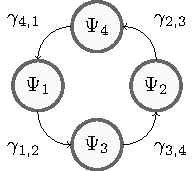
\includegraphics[width=0.3\textwidth]{berry_loop}
  \caption{Diagram illustrating the}
  \label{fig:berry_loop}
\end{figure}

\subsection{The Continuous Case \label{ssec:continuous_case}}

The most intuitive way to extend The Berry Phase to the continuous regime is by analogy to the discrete case. This will not be conducted in the manner of a formal mathematical proof showing that the same concepts introduced in the discrete case (\ref{ssec:discrete_case}) can be extended to the continuum, for such a proof please refer to \cite{Asboth2016}.\\

In the discrete case there were three fundamental components that were not explicitly identified, though were the key ingredients in allowing us to define The Berry Phase. These were as following:

\begin{itemize}
  \item The unique identifiers that we used to distinguish the various states within the Hilbert Space from one another. We will call the set of all identifiers the parameter ppace and denote this with $\mathbb{P}$. In the discrete case this set was given by the natural numbers $\mathbb{N}$.
  \item A unique mapping from the parameter space ($\mathbb{P}$) to the Hilbert space of our quantum system ($\mathcal{H}$). In the discrete case the wave function was given by $\Psi: \mathbb{N} \rightarrow, \quad n \mapsto \ket{\Psi_{n}}$. 
  \item A path. The path will be denoted with the variable $\mathcal{C}$. In the discrete case this was simply a sequence $[n_0, n_1, \ldots, n_m]$. 
\end{itemize}

By identifying these components we have broken down the search for The Berry Phase in the continuous regime down to the identification of the appropriate analogues for each of components identified above:

\begin{itemize}

  \item The first of which, the Parameter Space, is implicit in the nature of our question "how does one extend The Berry Phase to continuous Hilbert Spaces?": an n-dimensional continuous parameter space ($\mathcal{M}$).
  \item The wave function follows, being simply a mapping from the elements of the parameter space to the Hilbert Space: $\Psi: \mathbb{P} \rightarrow \mathcal{H}, \quad \bm{R} \mapsto \ket{\Psi(\bm{R})}$

  \item A path in a continuous space can no longer be described by a finite sequence and this concept must be expanded to the continuous realm:
  $\mathcal{C}: [0, 1] \rightarrow \mathbb{P}, \quad t \mapsto \bm{R}(t)$
\end{itemize}

Having translated the components required to define The Berry Phase in the discrete case to the continuous realm it is now possible to postulate an expression for this phase when working with a continuous Hilbert Space. In the discrete case The Berry Phase is given as the sum of the relative phases of each wave function connected by the path $\mathcal{C}$:

\begin{equation*}
\gamma(\mathcal{C})) = \sum_{i = 0}^{N} \gamma_{n_{i \; \mathrm{mod} \; N}, n_{i+1 \; \mathrm{mod} \; N}} 
\end{equation*}

In the continuum, since states live infinitely close together we have to consider all terms of the form $\lim_{dt \to 0}\gamma_{\mathcal{C}(t), \mathcal{C}(t + dt)}$ in the \textit{summation}. The continuous \textit{summation} of a given term is realized by an integral of the term divided by the measure of the space over which it is integrated.

\begin{equation}\label{eq:berry_phase_analog}
  \gamma(\mathcal{C}) = \lim_{dt \to 0} \int_0^1 \gamma_{\mathcal{C}(t), \mathcal{C}(t + dt)} d \bm{t}
\end{equation}

The main advantage in this analogy is that we can see that The Berry Phase in a continuous Hilbert Space can be understood as the summation of the relative phases of infinitesimally close together states along a closed path.

\begin{tabular}{||l|l|l||}
\hline
&\textbf{Discrete} & \textbf{Continuous}\\
\hline
\textbf{Parameter Space ($\mathbb{P}$)} & $\mathbb{N}_{0}$ &  $\mathcal{M}$\\
\hline
\textbf{Wave Function ($\Psi$)} & $\Psi: \mathbb{P} \rightarrow \mathcal{H}, \quad n \mapsto \ket{\Psi_{n}}$ & $\Psi: \mathbb{P} \rightarrow \mathcal{H}, \quad \bm{R} \mapsto \ket{\Psi(\bm{R})}$ \\
\hline
\textbf{Path} ($\mathcal{C}$) &  $[n_{0}, n_{1}, \ldots, n_{N-1}]$ & $\mathcal{C}: [0, 1) \rightarrow \mathcal{M}, \quad t \mapsto \bm{R}(t)$\\
\hline
\textbf{Berry Phase} ($\gamma(\mathcal{C}$)) & $\sum_{i = 0}^{N} \gamma_{n_{i \; \mathrm{mod} \; N}, n_{i+1 \; \mathrm{mod} \; N}}$ & $\lim_{dt \to 0} \int_0^1 \gamma_{\mathcal{C}(t), \mathcal{C}(t + dt)} d \bm{t}$\\
\hline
\end{tabular}

While the form of the berry phase derived above (Eq: \ref{eq:berry_phase_analog}) is useful for relating it to the compact case it is not yet in its most compact form. Utilizing integration by substitution and the continuity of the parametrization of the path $\mathcal{C}$ and assuming that this path is parametrized with respect to the arc length, we can transform the integral to a closed path integral in the parameter space ($\mathcal{M}$).

\begin{equation*}
  \gamma(\mathcal{C}) = \lim_{d\bm{r} \to 0} \oint_{\mathcal{C}} \gamma_{\bm{R}, \bm{R}+d\bm{r}} d\bm{R}
\end{equation*}

For the limit to be appropriately defined in the parameter space we have to assure that we continue to take the relative phase of state pairs lying on the parametrized path:

\begin{align*}
d\bm{r} &\in M_{R} && M_{R} := \{\bm{r} \in \mathbb{M}|\; \bm{R} + \bm{r} \in \mathcal{C}([0, 1])\}\\
\end{align*}

The limit can be taken by utilizing how the relative phase information is encoded into the Hilbert Space and taking the Taylor Expansion:


  \begin{equation*}
    \begin{aligned}
      &\lim_{d\bm{r} \to 0} \exp(-i \gamma_{\bm{R}, \bm{R + d\bm{r}}}) = 
       \lim_{d\bm{r} \to 0}\frac{\braket{\Psi(\bm{R})|\Psi(\bm{R} + d\bm{r})}}
       {|\braket{\Psi(\bm{R})|\Psi(\bm{R} +d\bm{r})}|}&\\
      &1 - i \gamma_{\bm{R}, \bm{R} + d\bm{r}} = \bra{\Psi(\bm{R})}(\ket{\Psi(\bm{R})} + \nabla_{\bm{R}} \ket{\Psi(\bm{R})})&\\
      &\Rightarrow \gamma_{\bm{R}, \bm{R + d\bm{r}}} =
       i\braket{\Psi(\bm{R})|\nabla_{\bm{R}}|\Psi(\bm{R})}
    \end{aligned}
  \end{equation*}

  with this we arrive at the most compact form of The Berry Phase in a continuous Hilbert Space:

  \begin{equation*}
    \gamma(\mathcal{C}) = \oint i \braket{\Psi(\bm{R})|\nabla_{\bm{R}}|\Psi(\bm{R})} d\bm{R}
  \end{equation*}

  The integrand of The Berry Phase in this form is known as The Berry Connection \cite{Asboth2016}. 
  
  \begin{equation*}
    \mathcal{A} := i \braket{\Psi(\bm{R})|\nabla|\Psi(\bm{R})}
  \end{equation*}

\section{Properties of The Berry Phase}

Having derived The Berry Phase for the continuous case we can begin analysing some of its various properties. Recalling that The Berry Connection takes on the role of measuring the relative phase difference between quantum states infinitesimally close together a natural first step would be to examine how this quantity behaves under gauge transformations.

  \begin{align*}
    \ket{\Psi(\bm{R})} &\rightarrow \exp(i \alpha(\bm{R})) \ket{\Psi(\bm{R})}\\
    \mathcal{A} &\rightarrow \mathcal{A} - \nabla \alpha(\bm{R})\\
  \end{align*}

  As we would expect this is a non-gauge invariant property. However following the same argumentation laid out in the discrete case, the next natural step is to see if we can find a formulation of The Berry Phase whose integrand is non-gauge invariant. This is achieved by utilizing Stokes Theorem on our expression for The Berry Phase.

  \begin{align*}
    \gamma(\mathcal{C}) &= \oint \mathcal{A} \cdot d\bm{R}\\
    & = \sum_{\mu, \nu} \int_{\mathcal{S}(\mathcal{C})} \frac{1}{2} \partial_{\mu} \mathcal{A}_{\nu} - \partial_{\nu} \mathcal{A}_{\mu} dR^{\mu} \wedge dR^{\nu}&
  \end{align*}


The integrand arising in this expression defines a second order tensor known as The Berry Curvature.

  \begin{equation*}
    \Omega_{\mu, \nu}(\bm{R}) := \partial_{\mu} \mathcal{A}_{\nu} - \partial_{\nu} \mathcal{A}_{\mu}  
  \end{equation*}

Examining this quantity for gauge-invariance utilizing the transformation rules for the Berry Connection derived above (\ref{}) we retrieve:


       \begin{align*}
         &\ket{\Psi(\bm{R})} \rightarrow \exp(i\alpha(\bm{R}))\ket{\Psi(\bm{R})}\\
         &\Omega_{\mu, \nu}(\bm{R}) \rightarrow \partial_{\mu} (\mathcal{A}_{\nu}
         - \partial_{\nu} \alpha(\bm{R})) - \partial_{\nu}(\mathcal{A}_{\mu} -
         \partial_{\mu} \alpha(\bm{R})) = \Omega_{\mu, \nu}(\bm{R})
      \end{align*}

confirming the gauge-invariance of this property.

\subsection{Magnetic Analogies}

As so far we have derived a handful of interesting quantities for a general continuous Hilbert Space. The Berry Phase we have shown is a gauge-invariant quantity which ultimately is a geometric property of the closed path over which it is defined in parameter space. The Berry Connection is the non-gauge invariant property which is related to The Berry Phase through an integral of the connection over a closed path. Finally, The Berry Curvature which is related to The Berry Connection through its \textit{cross-product} and gives The Berry Phase through integration of it through any surface bounded by a given path. These relationships have a one-to-one similarity to the classical relationships between another set of three quantities known throughout physics, namely; the magnetic flux ($\Phi$), The magnetic vector potential ($\bm{A}$), and the magnetic flux density field ($\bm{B}$).


    \begin{minipage}{0.4\textwidth}
       \begin{align*}
         \textbf{Phase:}&\\
         \gamma(C) &= \oint \bm{\mathcal{A}} \cdot d\bm{R} \\
                   &= \int_{\mathcal{S}(\mathcal{C})} 
                      \nabla \times \bm{\mathcal{A}} \cdot d\bm{s}\\
                   &= \int_{\mathcal{S}(\mathcal{C})} \bm{\Omega} \cdot d\bm{s}
       \end{align*}
    \end{minipage}
    \hspace{0.05\textwidth}
    \begin{minipage}{0.4\textwidth}
      \begin{align*}
        \textbf{Flux:}&\\
        \Phi(C) &= \oint \bm{A} \cdot d\bm{R} \\
                &= \int_{\mathcal{S}(\mathcal{C})}
                   \nabla \times \bm{A} \cdot d\bm{s} \\
                &= \int_{\mathcal{S}(\mathcal{C})} \bm{B} \cdot d\bm{s}
      \end{align*}
    \end{minipage}

\section{The Adiabatic Theorem}\label{sec:adiabatic_theorem}

Up until this point The Berry Phase has been introduced as a purely mathematical construct arising as a result of the geometry of continuous Hilbert Spaces \ref{}. There is of course no fundamental guarantee that there is any physical system that simulates the transformations to a given state which are necessary in order to translate this mathematical construct into a physical quantity. In this section we will discuss a fundamental example where this occurs known as The Adiabatic Theorem.\\

The Adiabatic Theorem is a statement pertaining to the \textit{slow} evolution of quantum systems, though adiabatic behaviour is a concept that extends well beyond the quantum realm. Adiabatic behaviour, in general, is the idea that so long as the environment of any given system changes \textit{slowly} enough (with respect to its internal dynamics) then the system will continue to exhibit the predictable behaviour solely determined by that of the internal system and the instantaneous\footnote{The external \textit{instantaneous} parameters will of course always influence the internal system, the postulate of adiabatic behaviour is that one does not have to keep track of its' \textit{dynamics} in the appropriate limit.} parameter values of the environment \cite{Griffiths2017}. The Adiabatic Theorem tailors this postulate to the quantum realm; defining what exactly it means for the parameters defining a quantum system to evolve sufficiently slowly, and describing how exactly the quantum time evolution is effected by this slow change of parameters in the adiabatic limit. It states:\\

\colorbox{lightgray}{
\begin{minipage}{0.9\textwidth}
\noindent\textbf{Theorem:}\\
\\
If $H(t)$, $0 \leq t \leq 1$ is  family of Hermitian Hamiltonians and if $E_n(t)$, $E_m(t)$ designate smooth functions of $t$ which are simple eigenvalues of $H(t)$ isolated from the rest of the spectrum, the state of a quantum system \[\Psi(t) = \sum_{n} c_{n}(t)\ket{n(t)}\] given by the time-dependent Schrödinger equation
  \[i\frac{d}{dt}\Psi_{T} = H(\frac{t}{T})\Psi_{T}(t)\]
evolves such that the amplitudes of the instantaneous eigenstates composing the wave function are given by:
    \begin{align*} 
        c_{n}(t) = c_{n}(0)e^{i\theta_{n}(t)}e^{i\gamma_{n}(t)} &&
        \theta_{n}(t)  &= -\hbar^{-1} \int_{0}^{t} E_{n}(t^{\prime}) dt^{\prime}\\  
        && \gamma_{n}(t) &= i\int_{0}^{t} \braket{n(t^{\prime})|\dot{n}(t^{\prime})}
        dt^{\prime}
    \end{align*}
as $T \to \infty$ \cite{Born1928, Berry1984, Simon1983, Sakurai1994}.
\end{minipage}
}

The proof of this theorem can be carried out in three parts:\\  

First we can derive a differential equation for the amplitudes of the individual eigenstates utilizing the time-dependent Schrödinger equation
      \begin{align*}
        &i\hbar\ket{\dot{\Psi}(t)} = \bm{H}(\frac{t}{T})\ket{\Psi(t)} && \text{Schrödinger equation}&\\
        &i\hbar \sum_{n} \left[ \dot{c}_{n}(t)\ket{n(t)} + c_{n}(t)\ket{\dot{n}(t)} \right] = \sum_{n} c_{n}(t) E_{n}(t) \ket{n(t)}&& \text{Linear expansion}&\\
        &i\hbar \dot{c}_{m}(t) + i \hbar \sum_{n} \braket{m(t)|\dot{n}(t)}
          = c_{m}(t) E_{m}(t)&& \text{Inner product with $\bra{m(t)}$ (*)}
      \end{align*}
Then we can utilize the time-independent Schrödinger equation to retrieve an expression that helps to simplify the differential equation above.
      \begin{align*}
        &\bm{H}(\frac{t}{T})\Psi(t) = \sum_{n}c_{n}(t)E_{n}(t)\ket{\Psi_{n}(t)} && \text{time-independent S.E.} &\\
        &\frac{1}{T}\dot{\bm{H}}(t) \ket{n(t)} + \bm{H}(\frac{t}{T}) \ket{\dot{n}(t)} = \dot{E}_{n}(t) \ket{n(t)} + E_{n}(t) \ket{\dot{n}(t)}&& \text{Apply $\partial_{t}$} &\\
         &\braket{m(t)|\frac{1}{T}\dot{\bm{H}}(t)|n(t)} + E_{m} \braket{m(t)|\dot{n}(t)} 
         =  E_{n}(t) \braket{m(t)|\dot{n}(t)}&& \text{Inner product with $\bra{m(t)}$}&\\
         &\braket{m(t)|\dot{n}(t)} 
         = \frac{\braket{m(t)|\frac{1}{T}\dot{\bm{H}}(t)|n(t)}}{E_{n}(t) 
         - E_{m}(t)} \quad (m \neq n)&& \text{Rearrange (**)}&\\
       \end{align*}
Finally we insert the result from the time-independent equation into those of the time-dependent equation and utilize the assumptions of the theorem to solve the resulting differential equation.
      \begin{flalign*}
        &\dot{c}_{m}(t) + \left( \frac{i}{\hbar} E_{m}(t) + \braket{m(t)|\dot{m}(t)} \right) c_{m}(t) =  \sum_{\substack{n\\ n \neq m}} \frac{\braket{m(t)|\frac{1}{T}\dot{\bm{H}}(t)|n(t)}}{E_{m}(t) - E_{n}(t)}&& \text{(**) into (*)}&\\
        &\dot{c}_{m}(t)  
        = i \left( - \frac{1}{\hbar}E_{m}(t) + i\braket{m(t)|\dot{m}(t)} \right)
        c_{m}(t)&& \text{limit as $T \to \infty$} &\\
        &c_{m}(t) 
        = c_{m}(0) e^{-i \frac{1}{\hbar} \int_{0}^{t} E_{m}(t^{\prime}) dt^{\prime}}
        e^{i\int_{0}^{t} i\braket{m(t^{\prime})|\dot{m}(t^{\prime}}dt^{\prime}}&& \text{Solve} &\\ 
      \end{flalign*}

In the above proof we see that the role of sufficient slowness and the concept of the adiabatic limit in the quantum realm is given by:
$\sum_{\substack{n\\ n \neq m}} \frac{\braket{m(t)|\frac{1}{T}\dot{\bm{H}}(t)|n(t)}}{E_{m}(t) - E_{n}(t)}$
In other words the timescale over which one must traverse a given family of Hamiltonians for the adiabatic approximation to hold, must be so long that at all time points the factor given by the sum is negligibly small with respect to the timescale of the evolution. The question remains however where does the geometric phase factor arise?\\

There are two phase factors that arise in this theorem: 

\begin{itemize}

  \item The first phase factor $\theta_{m}(t)  = -\hbar^{-1} \int_{0}^{t} E_{m}(t^{\prime}) dt^{\prime}$ is simply a result of the evolution of the Eigenenergy of the m-th state; initialization of the state in an eigenstate and solving the time-dependent Schrödinger equation retrieves this factor.

  \item The second phase factor $\gamma_{m}(t) = i\int_{0}^{t} \braket{m(t^{\prime})|\dot{m}(t^{\prime})} dt^{\prime}$ is less trivial then the \textit{dynamic phase} above and can be shown to be The Berry Phase. This is done by assuming that the time evolution of the Hamiltonian is mediated by a number of control parameters represented by some n-dimensional vector $\bm{R}$ 

  \begin{equation*}
    \bm{H}(t) = \bm{H}(\bm{R}(t)) \quad \Psi(t) = \Psi(\bm{R}(t))
  \end{equation*}

  \begin{flalign*}
    \gamma &=  \int_{0}^{t} i \braket{m(\bm{R}(t))|\dot{m}(\bm{R}(t))} dt&& \text{Specify dependency on $\bm{R}$}&\\
           &=  \int_{0}^{t}
    i \braket{m(\bm{R}(t))|\nabla_{\bm{R}}|m(\bm{R}(t))} \dot{\bm{R}}(t) dt && \text{Chain rule}&\\
           &= \oint i \braket{m(\bm{R})|\nabla_{\bm{R}}|m(\bm{R})}d\bm{R} && \text{Substitution}&\\
  \end{flalign*}

  Whereby we then recover the same expression for the Berry phase that we derived in Section \ref{ssec:continuous_case}.
\end{itemize}

\section{Physical Systems}\label{sec:physical_systems}
\subsection{Magnetic Moment in a Precessing Field}\label{ssec:magenetic_moment}

While the adiabatic theorem is clearly broadly applicable to a broad range of quantum physical phenomena and thus we can expect to find the geometric phase in a wide range of systems, it is of course prudent to prescribe the theory discussed in the last section (Sec: \ref{sec:adiabatic_theorem}) to a concrete system for which we can then calculate the corresponding geometric phase. To this end we will examine a spin-1/2 system under the influence of a magnetic field, changing in direction though not in magnitude.
  
  \begin{figure}
    \label{fig:spin_system}
    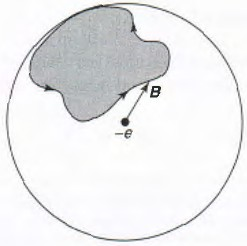
\includegraphics[width=0.3\textwidth]{b_spin_system_2}
    \caption{Motion of a 1/2-spin in an adiabatically changing magnetic field.}
  \end{figure}

A full description of the system is achieved by parametrizing the motion of the magnetic field in spherical coordinates and inserting it into the Hamiltonian describing the system.
      \begin{align*}
        \bm{B}(t) = B_{0} \begin{pmatrix} 
                                          \sin\theta(t)\cos\phi(t)\\
                                          \sin\theta(t)\sin\phi(t)\\
                                          \cos\theta(t)
                           \end{pmatrix}
        && \bm{H}(t) = \frac{\hbar e}{2m}\bm{B} \cdot \bm{\sigma}
      \end{align*}
The eigenstates of this Hamiltonian consist of the well known \textit{spin-up} and \textit{spin-down} wave functions for a magnetic field directed along a arbitrary axis in space. 
      \begin{align*}
        \chi_{+}(t) &= \begin{pmatrix} 
                                      \cos\frac{\theta(t)}{2}\\
                                      e^{i\phi(t)} \sin \frac{\theta(t)}{2}
                       \end{pmatrix} 
                       && E_{+} = \frac{\hbar \omega_{1}}{2}\\
       \chi_{-}(t) &= \begin{pmatrix} 
                                     e^{-i\phi(t)}\sin\frac{\theta(t)}{2}\\
                                     -\cos\frac{\theta(t)}{2}
                       \end{pmatrix} 
                       && E_{-} = -\frac{\hbar \omega_{1}}{2}
      \end{align*}

We thus see that the control parameters defining the evolution of our quantum system are given by the spherical coordinates $r, \theta, \phi$.\\

According to the adiabatic theorem (See:\ref{}) the calculation of the end state of the system is given by simple calculation of the dynamic and geometric phase factors of each eigenstate comprising the state in which our quantum system was initialized. Furthermore, if we evolve the quantum system adiabatically along a closed path then the geometric phase factor will correspond to the gauge-invariant Berry Phase. For this system we can then calculate The Berry Phase for an adiabatically changing system by direct integration of The Berry Connection along the path chosen in the spherical coordinate space:
  \begin{align*}
    &\gamma = \int_{\mathcal{C}} i \braket{\chi_{+}|\nabla_{r, \theta, \phi}|\chi_{+}} \cdot
    d\bm{B}&\\
    &\braket{\chi_{+}|\nabla_{r, \theta, \phi}|\chi_{+}} = i \frac{\sin^{2}(\theta /
        2)}{r \sin(\theta)} \hat{\phi}
  \end{align*}
Or by integration of the corresponding Berry Curvature over the entire surface enclosed by the path.
  \begin{align*}
    &\gamma_{+} = \int_{\mathcal{S}(\mathcal{C})} i \nabla_{r, \theta, \phi} \times
     \braket{\chi_{+}|\nabla_{r, \theta, \phi}|\chi_{+}} \cdot d\bm{s}&\\
    &\nabla_{r, \theta, \phi} \times
      \braket{\chi_{+}|\nabla_{r, \theta, \phi}|\chi_{+}} = \frac{i}{2r^{2}}\hat{r}&\\
    &\gamma = -\frac{\Omega}{2}
   \end{align*}
Doing so gives us a wonderful geometric interpretation of The Berry Phase as simply half of the solid angle enclosed by the path of the magnetic field vector in its evolution. The berry phase as a function of the solid angle has a periodicity of $4\pi$ which must give us the solid angle of the entire space, i.e. the solid angle associated with our system remaining at a singular point in parameter space. This result is of course unsurprising, as the solid angle of a spherical parameter space is a well known constant, but it is nonetheless a good practice in showing how information of the parameter space is embedded within the berry phase.\\

We can now use the result to see how the geometry of the parameter space embeds itself in the adiabatic evolution of a general state. Calculating the berry connection for the \textit{spin-down} state we find:
\begin{equation*}
  \braket{\chi_{-}|\nabla_{r, \theta, \phi}|\chi_{-}} = -i \frac{\sin^{2}(\theta /
  2)}{r \sin(\theta)} \hat{\phi}
\end{equation*}
and thus $\gamma_{-} = -\gamma_{+}$. Taking now a general state on the Bloch-sphere and evolving the system along a closed path results in a geometric phase factor for each eigenstate in the superposition. Rearranging then yields the transformation rule for a general state undergoing a cyclic adiabatic transformation:

\begin{align*}
  \Psi_i &= \cos \frac{\theta}{2} \ket{+} + e^{-i\phi}\sin \frac{\theta}{2}\ket{-}\\
  \Psi_f &= e^{-i\gamma_{+}}\cos \frac{\theta}{2} \ket{+} + e^{-i(\phi + \gamma_{-})}\sin \frac{\theta}{2}\ket{-}\\
  \Psi_f &= \cos \frac{\theta}{2} \ket{+} + e^{-i(\phi + \Omega)}\sin \frac{\theta}{2}\ket{-}\\
  \phi &\rightarrow \phi + \Omega
\end{align*}
Here we can see so long as the solid angle enclosed by the solid angle is less then $2\pi$ the resulting state will physically distinguishable from the initial one following the transformation.\\

\subsubsection{Numerical Solution}

While an analytical solution of The Berry Phase of this system is possible over The Berry Curvature, complex paths will of course making defining the region over which to integrate increasingly difficult. For complex paths then, a numerical solution is of increasing necessity. To this end however the formulation of The Berry Phase as a path integral (Eq: \ref{}) is more fitting, as calculation of the solid angle of the path would require the definition and classification of both the interior and exterior points of any given path before calculation could commence utilizing, for example, a Monte-Carlo method.\\

A given path is generated by discretizing the theta ($\theta$) and ($\phi$) coordinates in the regions mapping to the unit sphere following a coordinate transformation back to a cartesian representation
\begin{equation*}
  \theta \in [0, \pi]  \qquad  \phi \in [0, 2\pi)
\end{equation*}
into a number of discrete points defined by the user. A path is then drawn on this grid starting from the North Pole ($(0,0)$) by successive user input. For each \textit{segment} of a path the user is prompted to choose a direction ($\hat{e}_{\theta}$, $e_{\phi}$) along which they would like to travel as well as for an angular distance ($\theta$, $\phi$) indicating how many degrees the user wishes to travel in the chosen direction. For each segment chosen by the user the program checks whether any previous segment shares a point with the current one, indicating intersections. If an intersection is found the input is refused, and the user is reminded that the path must meet up with the initial point ($(0,0)$) to form a closed path.\\

Following path generation the numerical calculation of The Berry Phase is straightforward, as the path points can be considered to be the points of a curve parametrized with respect to the arc length.

\begin{equation*}
  \mathcal{C}: [0,1] \rightarrow \mathbb{S}^{2}
\end{equation*}

Therefore the magnitude of the vector connecting consecutive points can be considered a first-order approximation of the distance between two consecutive points along the path, which corresponds to a first order approximation of the width of the interval between them in continuous parametrization.

\begin{equation*}
  \forall x, y \in \mathcal{C}([0, 1]), \; x = C(t_x), \; y = C(t_y): \; L(C([t_x, t_y])) = \int_{t_{x}}^{t_{y}}dt \approx ||y - x||
\end{equation*}

This means that we can use a Riemann-Sum to approximate The Berry Phase
\begin{equation*}
  \gamma_{+} = \sum_{i < |P|} \frac{sin^{2}(\theta_{i}/2)}{r_{i}\sin(\theta)}\hat{e}_{\phi_{i}} \cdot (\bm{x}_{i + 1} - \bm{x}_{i})
\end{equation*}
and that its not necessary to multiply by the interval width in the parameter space of the parametrization since this information is embedded in the vector $\bm{x}_{i + 1} - \bm{x}_{i}$.\\

We can check the accuracy of the numerical result by taking a simple path such as traversing from the \textit{North Pole} to the \textit{Equator}, then over 90 degrees in the azimuthal direction and back up to the starting position. Here the analytical result is (ignoring the sign).
\begin{equation*}
  \gamma = \frac{\pi}{4} \approx 0.78540
\end{equation*}
while the numerical result gives
\begin{equation*}
  \gamma = 0.79331
\end{equation*}
with discretized sphere represented by 256 equally spaced points in the interval $[0, \pi]$ for both the azimuthal and polar directions.

\begin{figure}
  \begin{minipage}{.48\textwidth}
    \centering
    \label{fig:berry_path}
    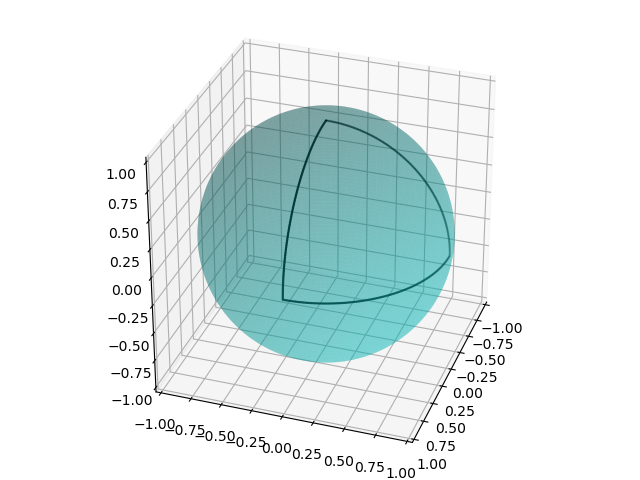
\includegraphics[width=\textwidth]{berry_phase_path_90_90_-90_256.png}
    \caption{Example closed path of a magnetic field vector along the unit sphere.}
  \end{minipage}%
  \hspace{2ex}
  \begin{minipage}{.40\textwidth}
    \centering
    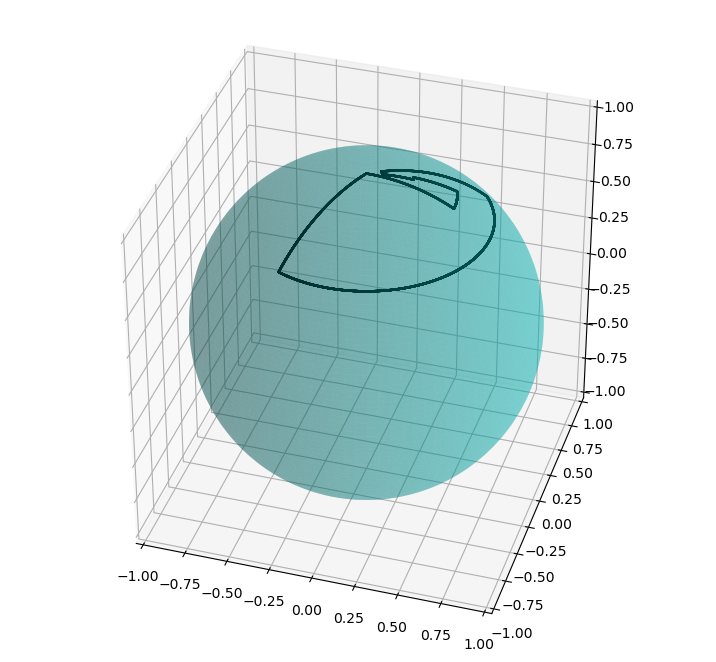
\includegraphics[width=\textwidth]{berry_phase_random_path.png}
    \caption{More complicated bath with a berry phase of $\gamma = 0.3609$ according to the numerical method}
    \label{fig:berry_path_random}
  \end{minipage}
\end{figure}

This of course can be improved by increasing the number of points used to represent the sphere and thus decreasing the distance of the points along any given path.

\begin{tabular}{||l|l|l||}
  \hline
  \textbf{256-Points} & \textbf{1024-Points} & \textbf{8192-Points}\\
  \hline
  0.79331 & 0.78737 & 0.78564\\
  \hline
\end{tabular}

\subsection{The Aharonov-Bohm Effect}\label{ssec:aharonov_bohm_effect}

While one of the most prominent examples of The Berry Phase arises during the adiabatic evolution of quantum systems it would be naive consider The Berry Phase an adiabatic effect. Looking back at theoretical discussions which kicked of this report in Section \ref{sec:the_berry_phase} it was clear that The Berry Phase arose due to internal phase relations of quantum states along a given path across the parameter space; the rate at which a given system underwent change did not enter into the discussion. One prominent effect where The Berry Phase arises and is not the result of the adiabatic change of a number of control parameters is the famous Aharonov-Bohm effect.\\

The Aharonov-Bohm effect was introduced in a paper by Yakir Aharonov and David Bohm in 1959. The paper put forward two physical systems showing that the electromagnetic potential was capable of acting upon particles independent of whether or not this corresponded with an observable electric or magnetic field. The two systems put forward came to be known as:

\begin{itemize}
  \item The electric Aharonov-Bohm effect, for the system demonstrating the physical effects of the electric scalar potential
  \item The magnetic Aharonov-Bohm effect, for the system demonstrating the physical effects of the magnetic vector potential.
\end{itemize}

This paper's significance lay in the fact that it called into question the physical relevance of the potentials which up until then had be considered useful mathematical constructs for representing the electric and magnetic fields. If it were to be maintained that the physically relevant quantities remained to be those simply of the E and B-fields then the concept of locality itself would have to be called into question; A field present in one region of space must effect the behaviour of a particle in another region from which it is seemingly expelled. On the other hand if it is maintained that the electromagnetic potential is indeed the fundamental quantity in a physical system then one has to grapple with the fact that exhibits a gauge-degree of freedom is somehow physical. It turns out that both of these effects can be elegantly explained as an example of The Berry Phase which we will show for each of these effects \cite{Aharonov1959}.

\subsubsection{The Electric Effect}\label{sssec:electric_effect}

 \begin{figure}[h]
   \centering
   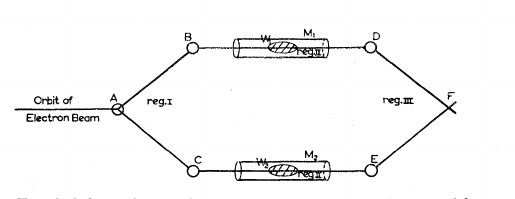
\includegraphics[width=0.6\textwidth]{electric_effect}
   \captionof{figure}{Electric effect schematic \cite{Aharonov1959}.}
   \label{fig:ABE}
 \end{figure}
 
The system in which the Electric Aharonov-Bohm effect arises is described by two sufficiently long parallel paths down which a particle beam of electrons can travel. Along each of these paths part of the path is shielded by the effects of an electric field by an idealized \textit{Faraday Cage}. One can consider a beam of electrons at some initial point \textbf{A} being split into two parts and travelling separately along each path. Once the electron beams have arrived at their respective Faraday Cages local time dependent electric fields are turned on. Then before each of the particle beams exits their respective Faraday Cages the local electric fields are turned off. Finally the beams are recombined at a later point \textbf{F} (See: \ref{fig:ABE}).\\

For a quantum mechanical description of this system we can write down the Hamiltonian
\begin{equation*}
  \bm{H} = \bm{H}_{0} + V(\bm{r},t)
\end{equation*}

Whereby $\bm{H}_{0}$ describes our system in the absence of any electric fields. We can specify the system further by restricting our space to the symmetrically split free state solutions travelling along the predefined paths through the Faraday Cages(i.e. the particle beams).
\begin{align*}
  \Psi_{0}(\bm{r},t)=\Psi_{L0}(x,t) + \Psi_{R0}(x,t) && \hat{\bm{X}}\Psi_{L0/R0} = \Psi_{R0/L0}
\end{align*}
In this restricted solution space the effect of two localized electric fields along each of the particle beam paths and one global field is indistinguishable. Therefore we can replace the global field operator with two localized operators acting solely along each of the paths which we will label Left ($L$) and Right ($R$).
\begin{align*}
  \bm{H} = \bm{H}_{0} + V_{L}(x,t) + V_{R}(x,t) && V|_{L/R} = V_{L/R}
\end{align*}
We further restrict the Hilbert Space of our unperturbed Hamiltonian ($\bm{H}_{0}$) to those states who are completely contained within the Faraday Cage during the entire duration that there exists an electric field. For such states we can disregard the spatial dependence of the potential since the potential within the region of the Faraday Cage is constant.
\begin{equation*}
  \bm{H} = \bm{H}_{0} + V_{L}(t) + V_{R}(t)
\end{equation*}
The effect of the time-dependent local electric field can be modelled by a time-dependent potential term; thus the complete Hamiltonian is given by:
\begin{equation*}
  \bm{H} = \bm{H}_{0} + V(\bm{r}, t) = \bm{H}_{0} + V_{L}(x,t) + V_{R}(x,t)
\end{equation*}
Under these assumptions the solution of the time-dependent Schrödinger equation can be achieved by solving the equation independently for each of the paths where the Hamiltonian becomes
\begin{align*}
  \bm{H}|_{L} &= \bm{H}_{0} + V_{L}(x,t)\\
  \bm{H}|_{R} &= \bm{H}_{0} + V_{R}(x,t)
\end{align*}
and thus the solution of the time-dependent Schrödinger equation along each of the paths is given by
\begin{align*}
  \Psi_{L/R} &= \Psi_{0} \exp(-i \mathcal{S}_{L/R})\\
  \mathcal{S}_{L/R} &= \int_{0}^{t} V_{L/R}(t^{\prime}) dt^{\prime} 
\end{align*}
that is the solution in the absence of any electric field ($\Psi_{0}$) times a phase factor given by the integral of the time dependent electric potential within the cage. It follows then that the quantum state of the entire system described then by the Hamiltonian
  \begin{equation*}
    \bm{H}(\bm{r}, t) = \bm{H}_{0} + V(\bm{r}, t)
  \end{equation*}
can be written as
\begin{equation*}
  \Psi(\bm{r})=\Psi_{L0}(x,t)\exp(-i \mathcal{S}_{L}) + \Psi_{R0}(x,t)\exp(-i \mathcal{S}_{R})
\end{equation*}
Clearly the phase terms appearing in the solution will result in noticeable interference upon their recombination. Interestingly enough however one can calculate The Berry Phase of this wave function by integrating along one path and back along the other
\begin{align*}
  \gamma &= \oint i\braket{\Psi|\nabla_{t,x}|\Psi} \cdot d\bm{r}\\
         &= \int_{L} i\braket{\Psi_{L}|\nabla_{\bm{r}}|\Psi_{L}} + \int_{R} i\braket{\Psi_{R}|\nabla_{\bm{r}}|\Psi_{R}} \cdot d\bm{r}\\
         &= S_{L} - S_{R}
\end{align*}
Thus the electric effect and the resulting interference of the two wave functions can be attributed to the geometry of the resulting Hilbert Space being enforced upon the wave functions travelling along their respective paths \cite{Aharonov1959}.

\subsubsection{The Magnetic Effect}\label{sssec:magnetic_effect}

\begin{figure}[h]
  \centering
  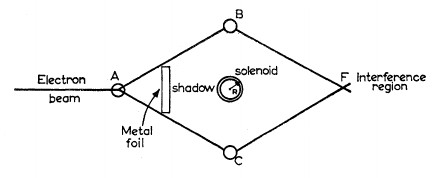
\includegraphics[width=0.6\textwidth]{magnetic_effect}
  \captionof{figure}{Magnetic effect schematic \cite{Aharonov1959}.}
  \label{fig:AME}
\end{figure}

The system in which the magnetic effect arises is very much similar to that of the electric effect and consists of a split electron beam forced along paths wrapping around a solenoid containing a finite flux, and then recombined at some further point.\\

In general the Hamiltonian of such a system can be written as:
\begin{equation*}
  \bm{H} = \frac{\left[ \bm{P} - \frac{e}{c}\bm{A} \right]^{2}}{2m} \\
\end{equation*}
After which one can follow the same argumentation followed in the last section (Sec: \ref{sssec:electric_effect}); restricting our Hilbert space to those regions describing symmetric beams, and replacing the global vector potential operator $\bm{A}$ with two local operators acting solely on the two paths $\bm(A)_{L/R}$ in order come up with a solution of the Hamiltonian
\begin{align*}
  \Psi(\bm{r})&=\Psi_{L0}(x,t)\exp(-i \mathcal{S}_{L}) + \Psi_{R0}(x,t)\exp(-i \mathcal{S}_{R})\\
  \mathcal{S}_{L/R} &= \int \bm{A} \cdot d\bm{x} 
\end{align*}
Since the form of this solution is fundamentally the same as the form of the solution found in the electric effect, we see that here as well that the phase factor arising in this system is an example of The Berry Phase \cite{Aharonov1959}.
  \begin{equation*}
    \gamma = \oint i\braket{\Psi|\nabla_{\bm{r}}|\Psi} \cdot d\bm{r} = S_{L} - S_{R}
  \end{equation*}

\bibliography{Zotero}
\bibliographystyle{plainnat}

\end{document}
